\chapter{Introduction}

%-------------------------------------------------------------------------------
% SECTION: Computer Graphics
%-------------------------------------------------------------------------------
\section{Computer Graphics}
Computer graphics is, in general, anything produced by a computer that isn't plain text or sound. Although, perhaps a more fitting definition is using a computer to draw a picture; this is also called rendering. There are a vast array of different areas in which one may want the help of a computer to render an image, from the entertaining, like video games and animated films, to the scientific, like medical visualization and computer-aided design and drafting. Each of these disciplines can have varying requirements of computer graphics: some need real-time rendering in order to respond to user-input, and others may trade the real-time speed for precise simulation. The goal of computer graphics is to identify the requirements of the application and render the highest quality image given those restrictions.

%-------------------------------------------------------------------------------
% SECTION: Ray-Tracing and Global Illumination
%-------------------------------------------------------------------------------
\section{Ray-Tracing and Global Illumination}
\label{sec:ray_tracing_intro}
In particular, this thesis is concerned with ray-traced rendering using Global Illumination algorithms, which are most commonly utilized to produce high-quality photo-realistic images. A ray-tracing algorithm can be classified as a Global Illumination algorithm when it incorporates not only direct illumination from light sources, but indirect illumination, or light that is inter-reflected between scene geometry from the same light sources (Figure \ref{fig:compare_illumination}).

\begin{figure}[h!]
    \centering
    \subfloat[Direct Only]{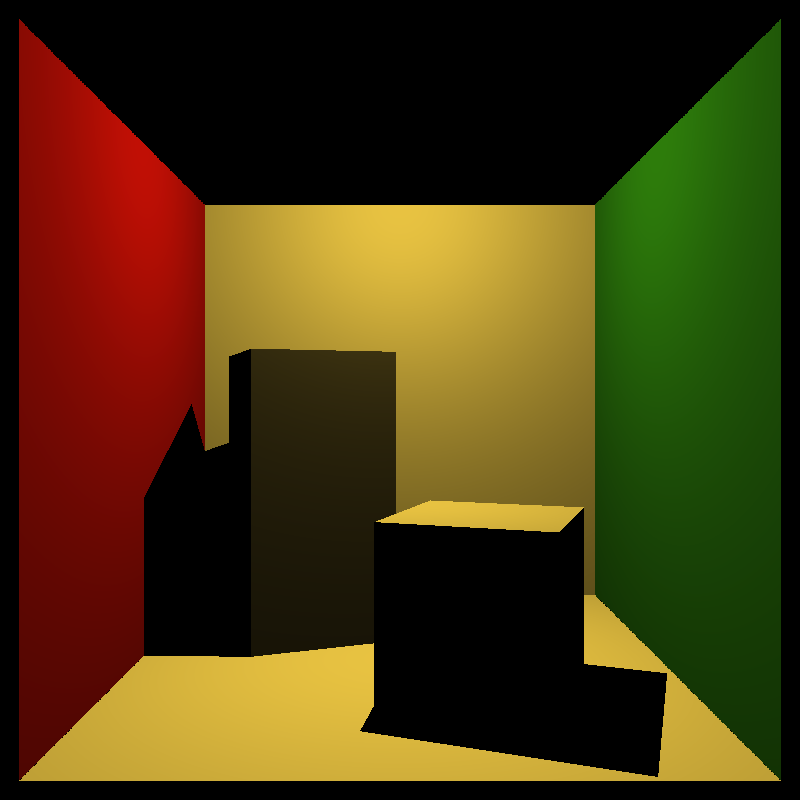
\includegraphics[width=70mm]{../img/cornell_simp_direct_only.png}}
    ~
    \subfloat[Direct \& Indirect]{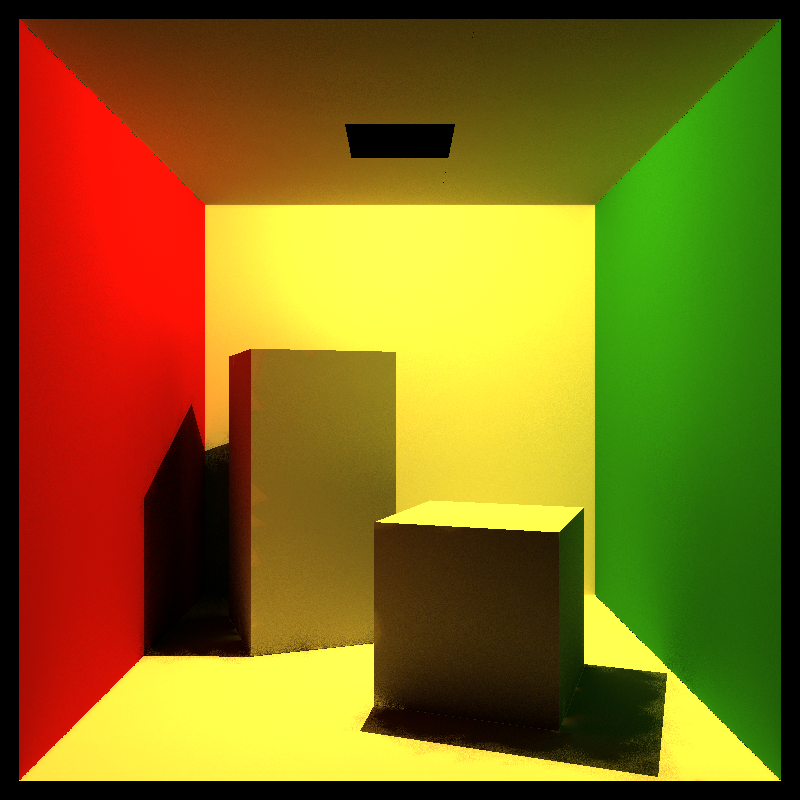
\includegraphics[width=70mm]{../img/cornell_simp_indirect.png}}
    \caption[Cornell Box direct \& indirect illumination]{Cornell Box rendered with both direct illumination and direct \& indirect illumination.}
    \label{fig:compare_illumination}
\end{figure}

Ray-tracing achieves photo-realism by simulating the physics of light using a scene comprised of light sources, mathematically-defined geometric surfaces, and a virtual camera (see figure \ref{fig:camera}). It produces renders that are specifically not real-time in nature, but meant to take as long as is necessary to produce quality results. In this setting, we must render life-like images, so an accurate simulation of light physics is required, but oftentimes we can obtain a convincing result using approximations. Specifically, ray-tracing follows the opposite path of the light: instead of tracing light rays from the light sources until they happen to hit the virtual camera, which is very physically accurate, we start at the camera and trace into the scene.

\begin{figure}[h!]
    \centering
    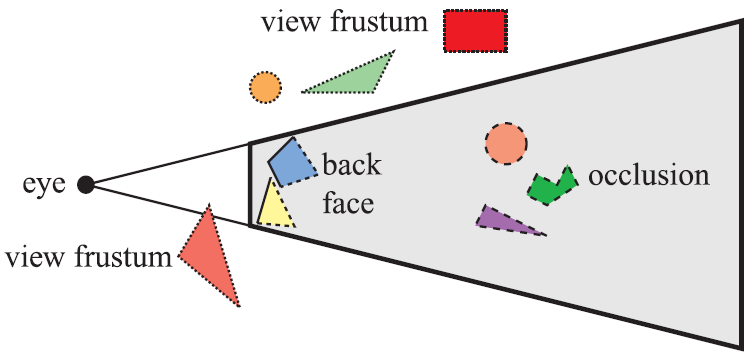
\includegraphics[width=100mm]{../img/RTR3_14_09_camera.png}
    \caption[Virtual camera, frustum, and geometry]{The eye and virtual camera are equivalent, geometry that lies in the viewing frustum is rendered. \cite{bib:rtr}}
    \label{fig:camera}
\end{figure}

Once these primary rays travel from the camera, into the scene, and intersect with the geometry, we can calculate the shading at that point in order to determine the color of the primary ray's associated pixel in the final rendered image. This shading calculation can vary from a simple direct illumination computation, to a complex Global Illumination calculation.

In this thesis, we focus on Global Illumination techniques. We split the calculation into direct illumination, which is the amount of light that leaves the source and directly intersects our shading point, and indirect illumination, which is the amount of light contributed from the diffuse inter-reflections of geometry in the scene; a phenomenon that is exemplified by the fact that the space under our desks is not completely dark, or that an illuminated red wall may reflect red light onto a nearby white box, causing it to appear reddish. These two components (direct and indirect illumination) are combined into one value that represents the incoming illumination at our primary ray's intersection point. We solve for the amount of this illumination that follows back along the ray to the camera, and we write that value to the primary ray's associated final-image-pixel. Performing this ray-tracing algorithm on each such final-image-pixel generates a rendering of the scene geometry as defined by the light sources and virtual camera, and is classified as Global Illumination.

%-------------------------------------------------------------------------------
% SECTION: Monte Carlo Ray-Tracing
%-------------------------------------------------------------------------------
\section{Monte Carlo Ray-Tracing}
\label{sec:monte_carlo}
One of the most widely used methods for the indirect illumination calculation in ray-tracing is called Monte Carlo sampling, and it involves randomly and discretely sampling the hemisphere above an intersection point (Figure \ref{fig:monte_carlo}). This is performed by recursively tracing yet more rays into the scene in order to gather information about what geometry is nearby and what color it is shaded; this attempts to solve for the diffuse inter-reflections incident at an intersection point. 

\begin{figure}[h]
   \centering
   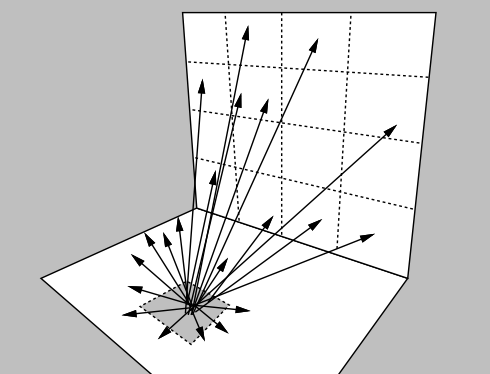
\includegraphics[width=80mm]{../img/shirley_monte_carlo.png}
   \captionfonts
   \caption[Monte Carlo hemisphere]{Monte Carlo sampling of a hemisphere above an intersection point \cite{bib:shirley1991}.}
   \label{fig:monte_carlo}
\end{figure}

Typically, around 128 of these rays are traced from each primary ray intersection point, into the scene, in order to gather enough shading information about the adjacent geometry to calculate a believable indirect illumination value. The number of rays that require intersection calculations, and shading calculations, can quickly escalate into the tens and hundreds of millions. Renders requiring multiple hours to complete are not rare.

%-------------------------------------------------------------------------------
% SECTION: Point-Based Color Bleeding
%-------------------------------------------------------------------------------
\section{Point-Based Color Bleeding}
Recently, the Point-Based Color Bleeding algorithm was developed at Pixar by Per H. Christensen \cite{bib:christensen2008} for indirect illumination. Instead of tracing rays, as in Monte Carlo ray-tracing, discretized surface elements (surfels) are rasterized onto a cube of eight-by-eight-pixel images, approximating the hemisphere used in the Monte Carlo ray-tracing (Figure \ref{fig:surfel_raster}). Once the surfels have been rasterized onto the pixels of the cube faces, the pixels are weighted and convolved into one value representing the indirect illumination at a point.

\begin{figure}[p]
   \centering
   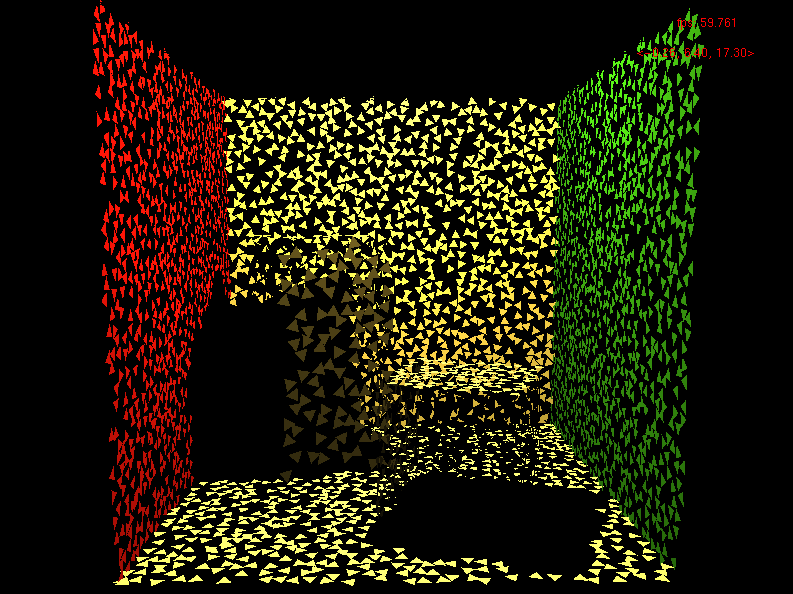
\includegraphics[width=130mm]{../img/surfel_cloud_tris.png}
   \captionfonts
   \caption[Cornell Box surfels]{Surfels for the Cornell Box scene. Note that the surfel size has been reduced to exhibit the sufel shape and distribution.}
   \label{fig:surfels}
\end{figure}

\begin{figure}[p]
   \centering
   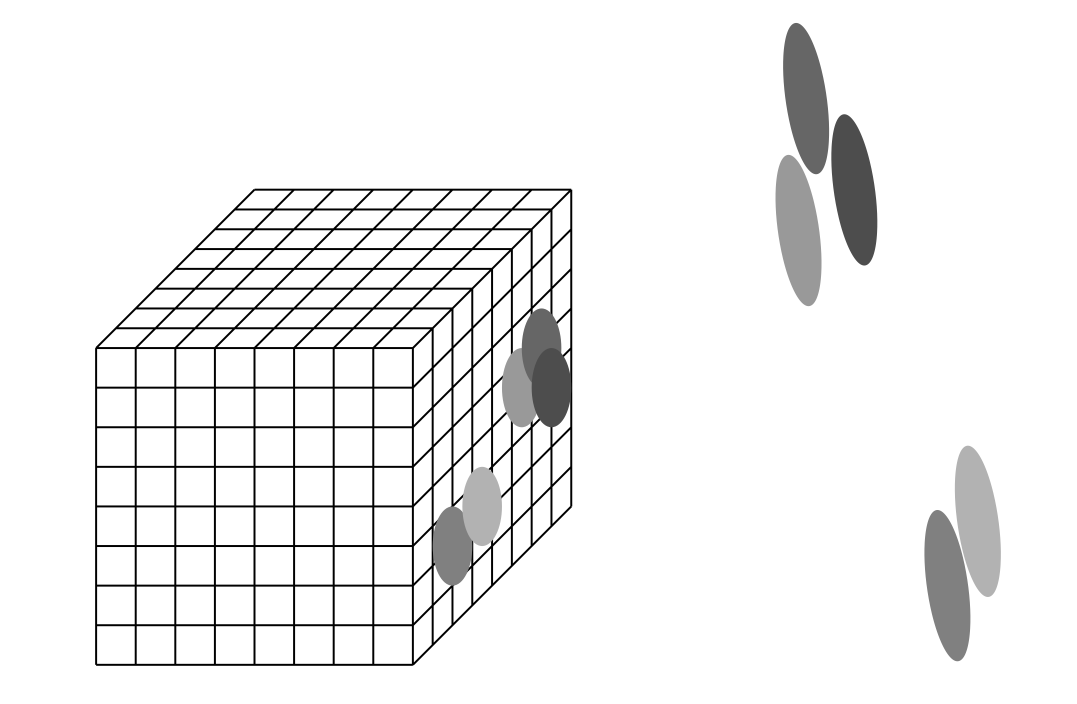
\includegraphics[width=100mm]{../img/surfel_raster.png}
   \captionfonts
   \caption[Rasterizing surfels]{Surfels being rasterized onto an 8x8 cube \cite{bib:christensen_slides}.}
   \label{fig:surfel_raster}
\end{figure}

The surfels are comprised of a location, surface normal, surface area, and shaded color computed from the direct illumination (Figure \ref{fig:surfels}). The benefit of this technique is that the surfels can be precomputed and stored in a point cloud, separate from the scene geometry, and reused. This lends itself well to reduced memory usage, surface shading independent run-time, and faster renders than Monte Carlo ray-tracing, all of which are very useful properties for Pixar and movie production in general.

%-------------------------------------------------------------------------------
% SECTION: Our Contribution
%-------------------------------------------------------------------------------
\section{Our Contribution}
This thesis is primarily concerned with performing the indirect illumination calculation faster than the Monte Carlo sampling method, without sacrificing render quality. We achieve this by extending PBCB to utilize the specialized rasterization capabilities of the modern heterogenous architecture chips' graphics processing unit (GPU) to rasterize the point cloud onto five eight-by-eight-pixel images arranged into a cube above each primary ray intersection point; this technique approximates the hemisphere that is used in the radiance integral (see section \ref{sec:radiance}). Also, we contribute a preprocess where the scene's geometry is transformed into triangles (the preferred geometric shape for GPU-rasterization) and assigned color values based on direct illumination calculations evaluated per triangle vertex.

\noindent In this paper, we:
\begin{itemize}
\item review important rendering related equations and techniques,
\item provide an in-depth description of the PBCB alrogithm,
\item present our PBCB extension and surfel generation preprocess,
\item discuss and analyze our validation techniques and results.
\end{itemize}

Our contributions, leveraging the modern heterogenous chips, realize much faster render times compared to Monte Carlo ray-tracing, while maintaining visually similar results (Figure \ref{fig:compare_techniques}). We achieve this by avoiding the numerous and costly intersection and shading calculations inherent in Monte Carlo Ray-tracing, and in some cases achieve an order of magnitude speedup.

\begin{figure}[h!]
    \centering
    \subfloat[Monte Carlo]{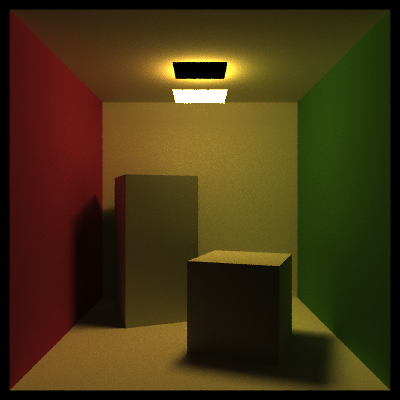
\includegraphics[width=70mm]{../img/cornell_simp_area_mcs.png}}
    ~
    \subfloat[GPU PBCB]{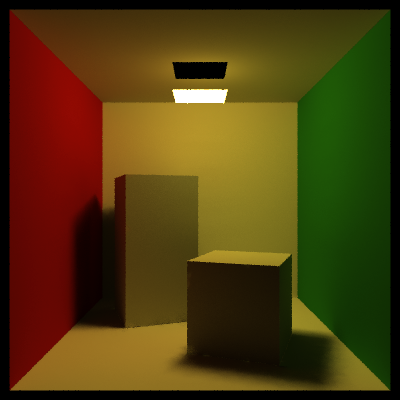
\includegraphics[width=70mm]{../img/cornell_simp_area_srf.png}}
    \caption[Cornell Box comparison]{Cornell Box with Indirect Illumination using both Monte Carlo Sampling and GPU PBCB.}
    \label{fig:compare_techniques}
\end{figure}

